\begin{figure}[htbp]
			\centering
			\begin{tikzpicture}[
				>=stealth,
				line cap=round,
				line join=round,
				]
				
				%------------------------------------------------------------
				% VINCOLO DI CERNIERA IN A
				%------------------------------------------------------------
				\draw[line width=1pt] (0,0)--(-0.4,-0.6)--(0.4,-0.6)--cycle;
				\draw[line width=0.8pt] (-0.50,-0.60)--(0.50,-0.60);
				\foreach \xi in {-0.40,-0.20,0.00,0.20}{
					\draw[thin] (\xi,-0.60)--(\xi-0.15,-0.85);
				}
				
				%------------------------------------------------------------
				% VINCOLO DI CARRELLO IN B
				%------------------------------------------------------------
				\draw[line width=1pt] (8,0)--(7.60,-0.60)--(8.40,-0.60)--cycle;
				\draw[line width=0.8pt] (7.50,-0.60)--(8.50,-0.60);
				\draw[line width=0.8pt] (7.75,-0.69) circle(0.09);
				\draw[line width=0.8pt] (8.25,-0.69) circle(0.09);
				\draw[line width=0.8pt] (7.50,-0.78)--(8.50,-0.78);
				\foreach \xi in {7.50,7.70,7.90,8.10,8.30}{
					\draw[thin] (\xi,-0.78)--(\xi-0.15,-1.03);
				}
				
				
				%------------------------------------------------------------
				% TRUSS
				%------------------------------------------------------------
				\draw[line width=1.5pt] (0,0)--(4,0)--(8,0);
				\draw[line width=1.5pt] (2,1.4)--(4,1.4)--(6,1.4);
				\draw[line width=1pt] (0,0)--(2,1.4);
				\draw[line width=1pt] (2,1.4)--(4,0);
				\draw[line width=1pt] (4,0)--(4,1.4);
				\draw[line width=1pt] (4,0)--(6,1.4);
				\draw[line width=1pt] (6,1.4)--(8,0);
				
				\foreach \x/\y in {0/0, 4/0, 8/0, 2/1.4, 4/1.4, 6/1.4}{
					\fill[white] (\x,\y) circle(3pt);
					\draw        (\x,\y) circle(3pt);
				}
				
				\node[above left,  font=\small] at (0,0)   {$A$};
				\node[below,       font=\small] at (4,0)   {$D$};
				\node[above right, font=\small] at (8,0)   {$B$};
				\node[above left,  font=\small] at (2,1.4) {$C$};
				\node[above right,       font=\small] at (4,1.4) {$E$};
				\node[above right, font=\small] at (6,1.4) {$F$};
				
				%------------------------------------------------------------
				% CARICO DISTRIBUITO
				%------------------------------------------------------------
				\draw (2,2.3)--(6,2.3);
				\foreach \x in {2, 2.67, 3.33, 4.00, 4.67, 5.33, 6.00}{
					\draw[->] (\x,2.3)--(\x,1.90);
				}
				\draw (2,1.90)--(6,1.90);
				\node[left, font=\small] at (2,2.10) {$q$};
				%		\draw (2,2.3)--(6,2.3);
				%		\foreach \x in {2, 2.67, 3.33, 4.00, 4.67, 5.33, 6.00}{
					%			\draw[->] (\x,2.3)--(\x,1.50);
					%		}
				%		\node[above, font=\small] at (4,2.3) {$q$};
				%		\draw[<->,thin] (2,1.95)--(6,1.95);
				%\node[above, font=\scriptsize] at (4,1.95) {$2d$};
				
				%------------------------------------------------------------
				% SEZIONE DI RITTER
				%------------------------------------------------------------
				\draw[dashed, line width=0.8pt]
				(5.3,1.9) .. controls (5.7,0.7) .. (5.3,-0.2);
				\node[right, font=\scriptsize] at (5.6,0.5) {sez.~Ritter};
				
				%------------------------------------------------------------
				% QUOTATURA ALTEZZA h
				%------------------------------------------------------------
				\draw[|<->|,thin] (-0.6,0)--(-0.6,1.4);
				\node[left, font=\small] at (-0.6,0.7) {$h$};
				\draw[thin] (-0.75,0)--(-0.45,0);
				\draw[thin] (-0.75,1.4)--(-0.45,1.4);
				
				%------------------------------------------------------------
				% QUOTATURA CON CAMPI d
				%------------------------------------------------------------
				\foreach \xa/\xb in {0/2, 2/4, 4/6, 6/8}{
					\draw[<->,thin] (\xa,-1.25)--(\xb,-1.25);
				}
				\foreach \x in {0,2,4,6,8}{
					\draw[thin] (\x,-1.17)--(\x,-1.33);
				}
				\node[above, font=\scriptsize] at (1,-1.25) {$d$};
				\node[above, font=\scriptsize] at (3,-1.25) {$d$};
				\node[above, font=\scriptsize] at (5,-1.25) {$d$};
				\node[above, font=\scriptsize] at (7,-1.25) {$d$};
				%\node[below=0.28cm, font=\small] at (4,-1.25) {$L=4d$};
				
				%------------------------------------------------------------
				% TRAVE EQUIVALENTE
				%------------------------------------------------------------
				%\node[font=\small, gray] at (4,-2.1) {trave equivalente};
				\draw[line width=1.5pt] (0,-2.4)--(8,-2.4);
				%\foreach \x in {0,2,4,6,8}{
					%	\fill[white] (\x,-2.4) circle(2.5pt);
					%	\draw        (\x,-2.4) circle(2.5pt);
					%}
				% carichi nodali equivalenti
				\draw[->] (2,-1.95)--(2,-2.35);
				\node[left, font=\small] at (2,-1.95) {$\tfrac{qd}{2}$};
				\draw[->] (4,-1.75)--(4,-2.35);
				\node[right, font=\small] at (4,-1.75) {$qd$};
				\draw[->] (6,-1.95)--(6,-2.35);
				\node[right, font=\small] at (6,-1.95) {$\tfrac{qd}{2}$};
				% reazioni
				\draw[->] (0,-2.85)--(0,-2.45);
				\node[left, font=\small] at (0,-2.85) {$qd$};
				\draw[->] (8,-2.85)--(8,-2.45);
				\node[right, font=\small] at (8,-2.85) {$qd$};
				
				%------------------------------------------------------------
				% DIAGRAMMA M_eq (positivo verso il basso)
				%------------------------------------------------------------
				\fill[gray!15]
				(0,-2.4)--(2,-3.65)--(4,-4.15)--(6,-3.65)--(8,-2.4)--cycle;
				\draw (0,-2.4)--(2,-3.65)--(4,-4.15)--(6,-3.65)--(8,-2.4);
				\draw[dashed,thin] (2,-2.4)--(2,-3.65);
				\draw[dashed,thin] (4,-2.4)--(4,-4.15);
				\draw[dashed,thin] (6,-2.4)--(6,-3.65);
				\node[left,  font=\small] at (2.7,-3.15) {$qd^2$};
				\node[below, font=\small] at (4.5,-2.85) {$\tfrac{3}{2}qd^2$};
				\node[right, font=\small] at (6,-3.15) {$qd^2$};
				\node[right, font=\small] at (8.2,-3.27) {$M_{\!\text{eq}}$};
				
				%------------------------------------------------------------
				% DIAGRAMMA T_eq
				%------------------------------------------------------------
				
				% +qd (A → C)
				\fill[gray!15] (0,-4.95)--(0,-4.45)--(2,-4.45)--(2,-4.95)--cycle;
				\draw (0,-4.95)--(0,-4.45)--(2,-4.45)--(2,-4.95);
				\node[above, font=\small] at (1,-4.45) {$+qd$};
				% +qd/2 (C → E)
				\fill[gray!15] (2,-4.95)--(2,-4.70)--(4,-4.70)--(4,-4.95)--cycle;
				\draw (2,-4.95)--(2,-4.70)--(4,-4.70)--(4,-4.95);
				\node[above, font=\scriptsize] at (3,-4.70) {$+\tfrac{qd}{2}$};
				% −qd/2 (E → F)
				\fill[gray!15] (4,-4.95)--(4,-5.20)--(6,-5.20)--(6,-4.95)--cycle;
				\draw (4,-4.95)--(4,-5.20)--(6,-5.20)--(6,-4.95);
				\node[below, font=\scriptsize] at (5,-5.20) {$-\tfrac{qd}{2}$};
				% −qd (F → B)
				\fill[gray!15] (6,-4.95)--(6,-5.45)--(8,-5.45)--(8,-4.95)--cycle;
				\draw (6,-4.95)--(6,-5.45)--(8,-5.45)--(8,-4.95);
				\node[below, font=\small] at (7,-5.45) {$-qd$};
				\node[right, font=\small] at (8.2,-4.95) {$T_{\!\text{eq}}$};
				% linea di riferimento del diagramma
				\draw[line width=0.7pt, black] (0,-4.95)--(8,-4.95);
				
				
				
			\end{tikzpicture}
			\caption{Travatura a correnti paralleli con carico
				distribuito sul corrente superiore. In alto:
				schema strutturale con sezione di Ritter
				tratteggiata nel pannello centrale. In basso:
				trave equivalente con diagrammi $M_\text{eq}$
				e $T_\text{eq}$.}
			\label{fig:travatura_correnti}
		\end{figure}
